\section{Differneces between 8086 \& 8088}
\begin{itemize}
  \item Virtually no difference between these two $\mu p$s. Both are packaged in 40-pin dual in-line packages (DIPs)
\end{itemize}
\begin{description}
  \item[8086] 16 bit $\mu p$ with a 16-bit data bus ($AD_0 - AD_{15}$)
  \item[8088] 16 bit $\mu p$ with a 8-bit data bus ($AD_0 - AD_7$)
\end{description}
8086 : $M/\overline{IO}$; 8088 : $IO/\overline{M}$;\newline
8086 (PIN 34): $\overline{BHE}/S7$; 8088 (PIN 34): $SSO$;\newline
\begin{description}
  \item[Power Supply Requirements]
  \begin{itemize}
    \item Both : $+5.0V$ with a supply voltage tolerance of $\pm 10\%$
    \item Both : $32^\circ F$ to $180^\circ F$
    \item 8086 : $360 mA$ ; 8088 : $340 mA$ (max supply current)
    \item CMOS version : 80C86 and 80C88 : $10 mA$ and $-40^\circ F$ to $225^\circ F$
  \end{itemize}
\end{description}
\newpage
\subsubsection{Pin diagram 8086}
\begin{figure}[h!]
    \centering
    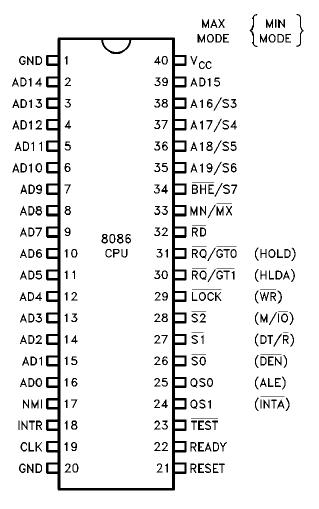
\includegraphics[width = 0.8\textwidth]{./figures/8086_MaxMode.jpg}
    \caption{Pin Diagram for Intel 8086 Max mode {Min Mode}}
    \label{fig:bl}
\end{figure}

\subsubsection{Pin diagram 8088}
\begin{figure}[h!]
    \centering
    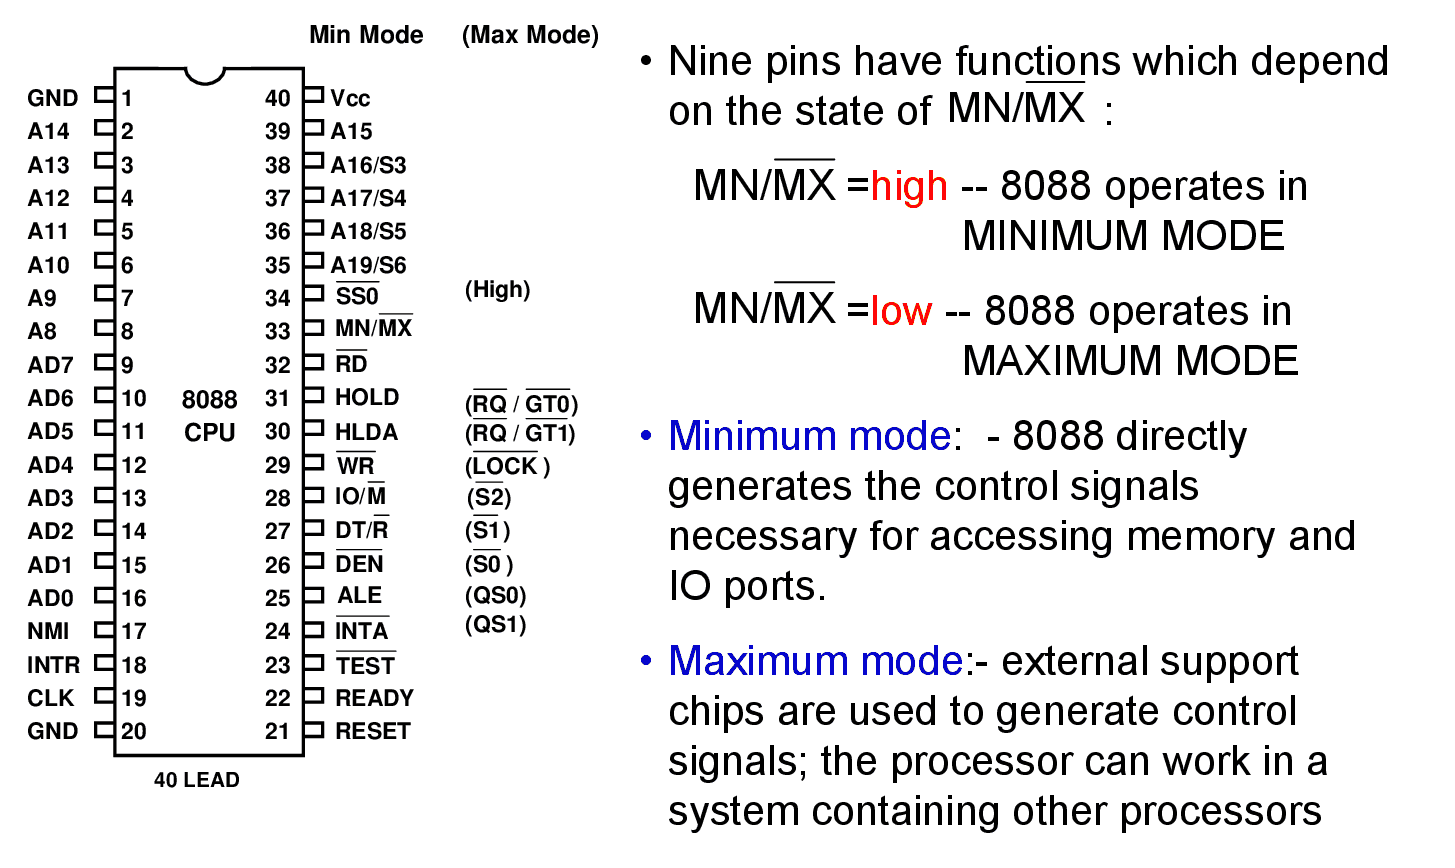
\includegraphics[width = 1.5\textwidth]{./figures/8088_MinMode.png}
    \caption{Pin Diagram for Intel 8088 Min mode {Max Mode}}
    \label{fig:bl}
\end{figure}

\section{Pin Connections}
\begin{description}
  \item[$AD_7 - AD_0$]
  \begin{itemize}
    \item 8088 address / data bus lines
    \item Multiplexed address data bus
    \item Rightmost eight bits of the memory address or I/O port no. whenever ALE is active (Logic 1) or data whenever ALE is inactive (Logic 0)
    \item High impedance state during a hold acknowledge
  \end{itemize}

  \item[$A_{15} - A_8$]
  \begin{itemize}
      \item  8088 address bus (upper half memory address bits)
      \item  High impedence state during a hold acknowledge.
  \end{itemize}

  \item[$AD_{15} - AD_8$]
  \begin{itemize}
      \item  8086 address/data bus lines
      \item  Contains address bits $A_{15} - A_8$, when ALE is logic 1
      \item Enter in high-impedence state whenever a hold acknowledge occurs.
  \end{itemize}

  \item[$A_{19}/S_6 - A_{16}/S_3$]
  \begin{itemize}
      \item  Multiplexed address/ status bus
      \item  Enter in high-impedence during hold acknowledge.
  \end{itemize}

  \item[$S_6$] Always 0
  \item[$S_5$] Indicates the condition of Interrupt flag
  \item[$S_4,S_3$] Indicate segment accessed during current bus cycle
  \begin{table}[h!]
  \centering
  \begin{tabular}{ |p{2cm}|p{2cm}||p{5cm}|  }
  \hline
  $S_4$ & $S_3$ & Function  \\
  \hline
  0 & 0  & Extra Segment\\
  0 & 1  & Stack Segment\\
  1 & 0  & Code or no segment\\
  1 & 1  & Data Segment\\
  \hline
  \end{tabular}

  \caption{Segment accessed during current Bus cycle}
  \label{table:1}
  \end{table}

  \item[$\overline{RD}$]
  \begin{itemize}
      \item  Whenever this pin goes to logic 0, the data bus becomes receptive to data from the memory or I?O devices
          connected to the system.
      \item Floats to high impedence state during a hold acknowledge
  \end{itemize}

  \item[READY]
  \begin{itemize}
      \item $\mu p$ enters into \textbf{WAIT} state and remains idle if this pin is at logic 0
      \item No effect on operations of $\mu p$, if this pin is at logic 1
  \end{itemize}


  \item[INTR]
  \begin{itemize}
      \item  Used to request a h/w interrupt
      \item  If INTR is held high when $IF = 1$, the $\mu p$ enters an interrupt acknowledge cycle
      ( $\overline{INTA}$ becomes active) after completion of the current instruction
  \end{itemize}

  \item[$\overline{TEST}$]
  \begin{itemize}
      \item  An input that is tested by the WAIT instruction
      \item  If TEST is logic 0, the WAIT instruction functions as NOP
      \item If TEST is logic 1, the WAIT instruction waits for \textbf{TEST} to become 0
  \end{itemize}

 \item[NMI]
 \begin{itemize}
     \item Non markable interrupt pin
     \item Similar to the \textbf{INTR} except that NMI does not check IF (whether it is 1)

 \end{itemize}

\end{description}
